% Описывается прикладная задача,
% параметры анализируемых данных (например, сколько объектов, сколько признаков, каких они типов),
% параметры эксперимента (например, как генерировались модельные данные, как производился скользящий контроль).
% Результаты экспериментов представляются в~виде таблиц и~графиков.
% Объясняется точный смысл всех обозначений на~графиках, строк и~столбцов в~таблицах.
% Приводятся выводы:
% в~какой степени результаты экспериментов согласуются с теорией?
% Достигнут ли желаемый результат?
% Обнаружены ли какие-либо факты, не~нашедшие объяснения,
% и~которые нельзя списать на «грязный» эксперимент?

% Цель данного раздела:
% продемонстрировать, что предложенная теория работает на практике;
% показать границы её применимости;
% рассказать о~новых экспериментальных фактах.

% Чисто теоретические работы могут не содержать данного раздела (на~практике не~работает, ну и~не~надо "--- зато теория красивая).
% Кстати, теоретики имеют право не догадываться, где, кому и~когда их~теории пригодятся.

Тестирование моделей мира проводилось в двух бенчмарках обучения с подкрепления, MetaWorld \cite{mtw} и CasualWorld \cite{cw}. 
Оба пакета предоставляют инструментарий для разработки и тестирования сред и алгоритмов обучения с подкреплениями, решающих задачу роботизированного контроля.

\subsection{Эксперименты в наборе сред MetaWorld}
Библиотека сред MetaWorld \cite{mtw} предоставляет широкие возможности для тестирования и сравнения алгоритмов мета-обучения и мультизадачного обучения и состоит из 50 задач, различающихся объектами, присутствующими в среде и целями, которые алгоритм должен достичь. Предлагаемые в работе архитектуры моделей мира в первую очередь рассчитаны на обобщение между задачами, имеющими одинаковую семантическую структуру, поэтому проверка алгоритма на всем наборе представляется неуместной. Также, некоторые из задач являются достаточно сложными даже для базового алгоритма, что представляло бы трудности в анализе обобщающей способности.

Для удобного тестирования предложенного подхода была создана новая среда, предлагаемое название которой RotatedDrawerOpen.
В ней содержится два объекта - шкаф с выдвижным ящиком и робот.
В конкретной задаче позиция шкафа закреплена, однако между задачами она меняется.
Примеры изображений различных задач среды представлены на рисунке \ref{fig:rdw}.

\begin{figure}[h]
    \centering
    \begin{subfigure}{.3\textwidth}
        \centering
        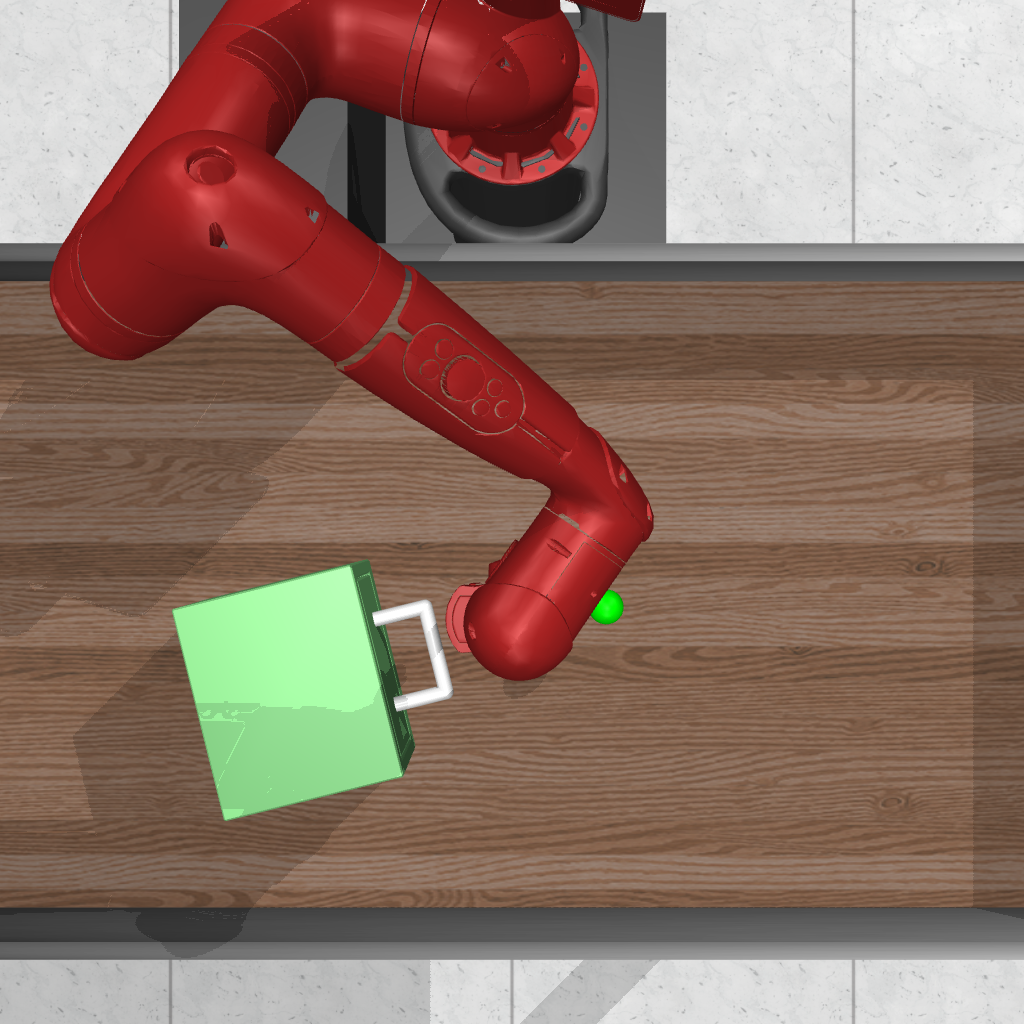
\includegraphics[width=\linewidth]{figures/pos1.png}
    \end{subfigure}
    \begin{subfigure}{.3\textwidth}
        \centering
        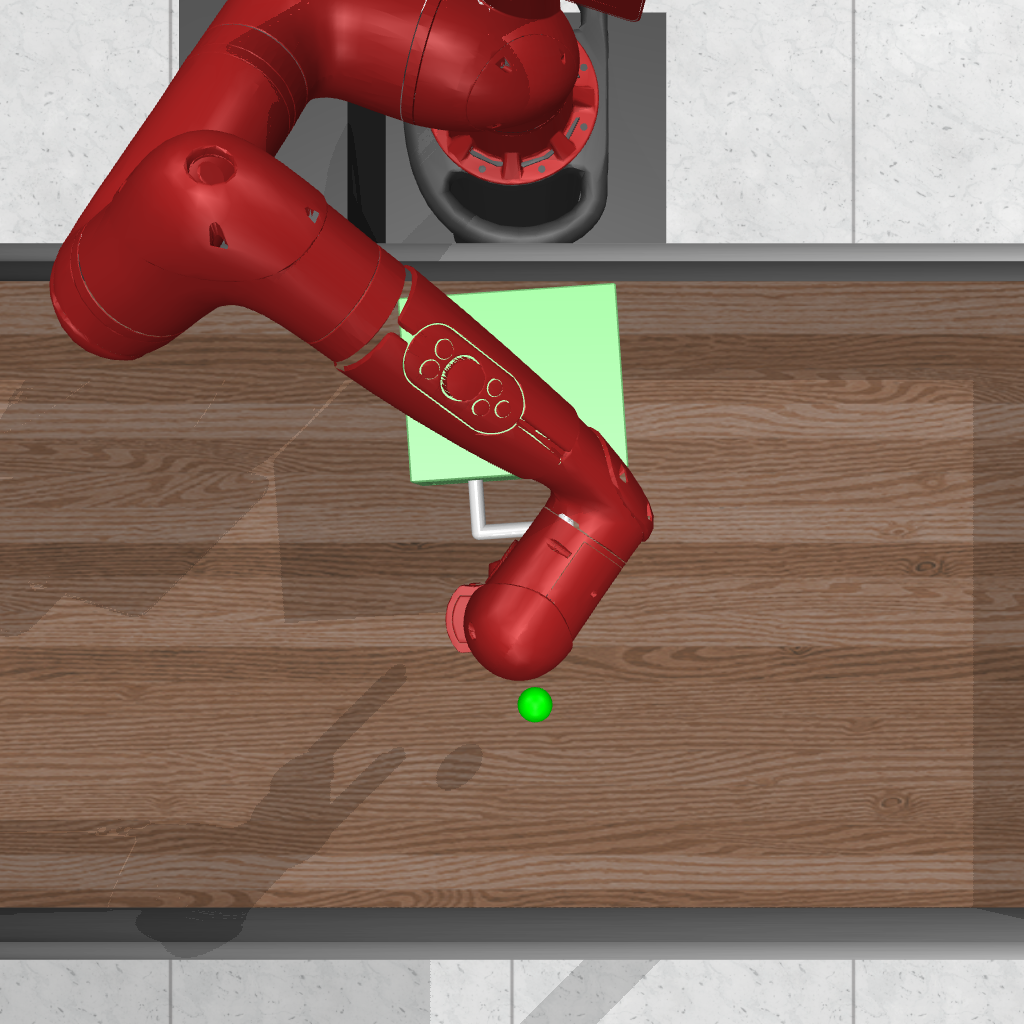
\includegraphics[width=\linewidth]{figures/pos2.png}
    \end{subfigure}
    \begin{subfigure}{.3\textwidth}
        \centering
        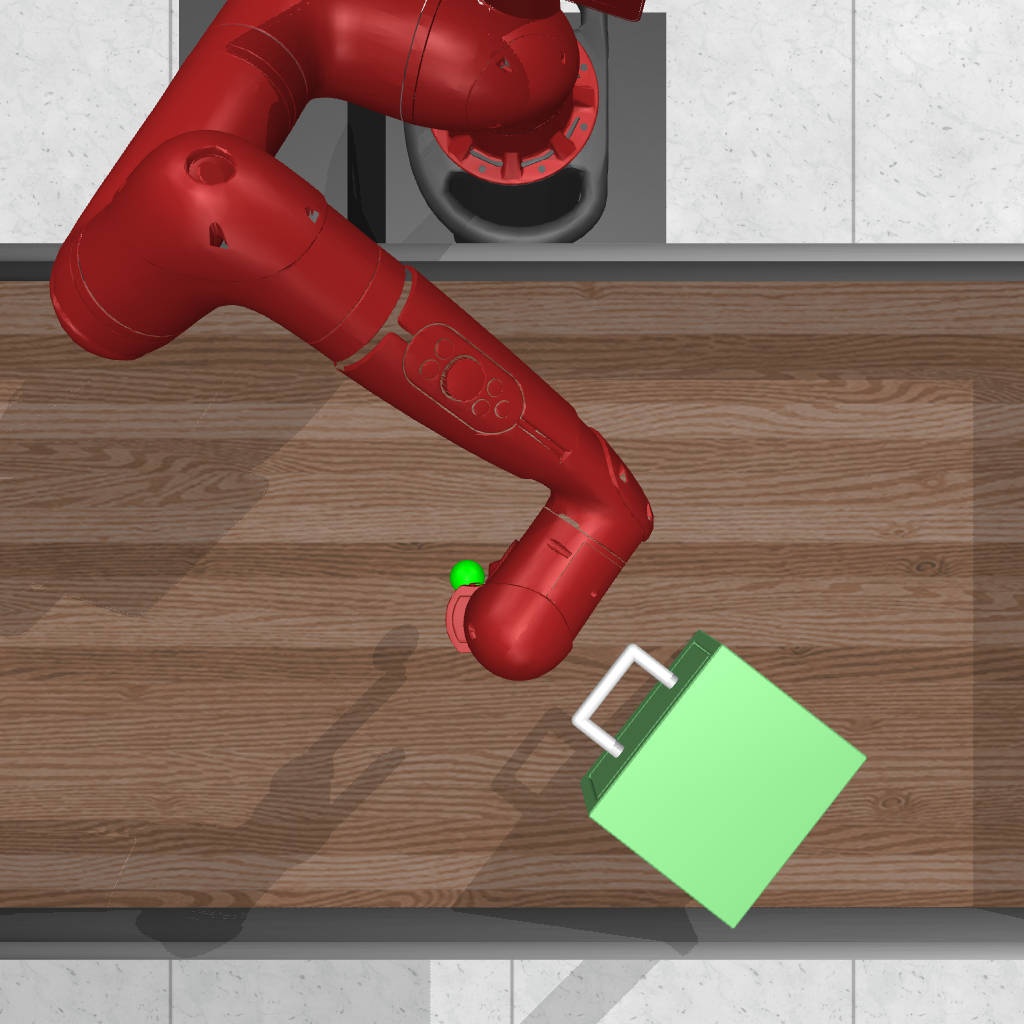
\includegraphics[width=\linewidth]{figures/pos3.png}
    \end{subfigure}
    \caption{Примеры задач в среде RotatedDrawerOpen.}
    \label{fig:rdw}
\end{figure}

Рассмотрим полярную систему координат с центром в середине сцены, в ней центр ящика имеет координаты $(R, \alpha_{\tau}, h)$.
Для всех задач значения координат $R$ и $h$ одинаковы и не меняются ни в течения эпизода, ни между задачами.
Множество задач, таким образом, совпадает с множеством значений $\alpha_{\tau}$ и равно $\left[0, 2\pi\right) \in \mathbb{R}$.
Контекст $c$ в экспериментах в этой среде определяется следующим образом:
\begin{equation}
    c = \alpha_{\tau}, \quad \forall{\tau} \in \mathcal{T}
\end{equation}
Множество задач $\mathcal{T}$ разделено на $\mathcal{T}_{\text{train}}$ и $\mathcal{T}_{\text{test}}$ следующим образом:
\begin{align}
    \mathcal{T}_{\text{train}} = & \{\tau \mid 
    \alpha_{\tau} \in \left[0, \frac{\pi}{4}\right) \cup \left[\frac{3\pi}{4}, \frac{5\pi}{4}\right) \cup
    \left[\frac{7\pi}{4}, 2\pi\right)\};
    \notag
    \\
    \mathcal{T}_{\text{test}} = & \{\tau \mid \alpha_{\tau} \in \left[\frac{\pi}{4}, \frac{3\pi}{4}\right) \cup \left[\frac{5\pi}{4}, \frac{7\pi}{4}\right)\}.
\end{align}
Разделение такого вида выбрано для уменьшения эффекта ухудшения работы энкодера на изображениях с еще не виденной позицией шкафа.
Действия $a \in \mathbb{R}^4$ представляют собой координаты следующего положения руки робота и число, регулирующее сжатие его пальцев.

На шаге $t$ агент получает получает из среды в качестве наблюдения робота $o_t$ и наблюдения объекта $o'_t$ сегментированные изображения робота и объекта соответственно.
Изображения являются тензорами размера $64 \times 64 \times 3$, камера для всех задач зафиксирована в одном положении сверху сцены.
Из-за подобного расположения камеры, сегментационная маска шкафа достаточно часто перекрыта изображением робота, в особенности в процессе выдвижения ящика.
Тогда как подобная ситуация вписывается в постановку задачи и должна решаться алгоритмом за счет рекуррентного вывода $q(s^o_{t+1} \mid s^o_{t}, u_t, o^o_{t+1})$, визуальные дефекты маски объекта могут мешать обучению объектной части модели мира, в особенности если вывод не рекуррентен $q(s^o_{t+1} \mid o^o_{t+1})$.
Чтобы исключить из анализа этот эффект, среда предоставляет в качестве объектного наблюдения $o^o_t$ сегментационную маску объекта, полученную из виртуальной копии среды без робота.
Функция награды не является разреженной и полностью соответствует функции награды из среды DrawerOpen пакета MetaWorld.

Подобная среда была выбрана для экспериментирования по нескольким причинам:
\begin{itemize}
    \item Каждая отдельная задача в среде является достаточно простой для базового алгоритма, что позволяет сфокусироваться на улучшении обобщающей способности без необходимости проводить долгий процесс обучения и модификации алгоритма под задачу.
    \item Все задачи в среде имеют одну и ту же структуру, зависящую от единственного параметра вариации, что делает полученные результаты более визуализируемыми и трактуемыми.
    \item Структура задач в среде позволяет алгоритму получить достаточно информации из единственной камеры с закрепленным положением, что избавляет агента от необходимости обрабатывать сложные 3-D композиции положений объекта.
\end{itemize}

\begin{figure}[t]
    \centering
    \begin{subfigure}{.47\textwidth}
        \centering
        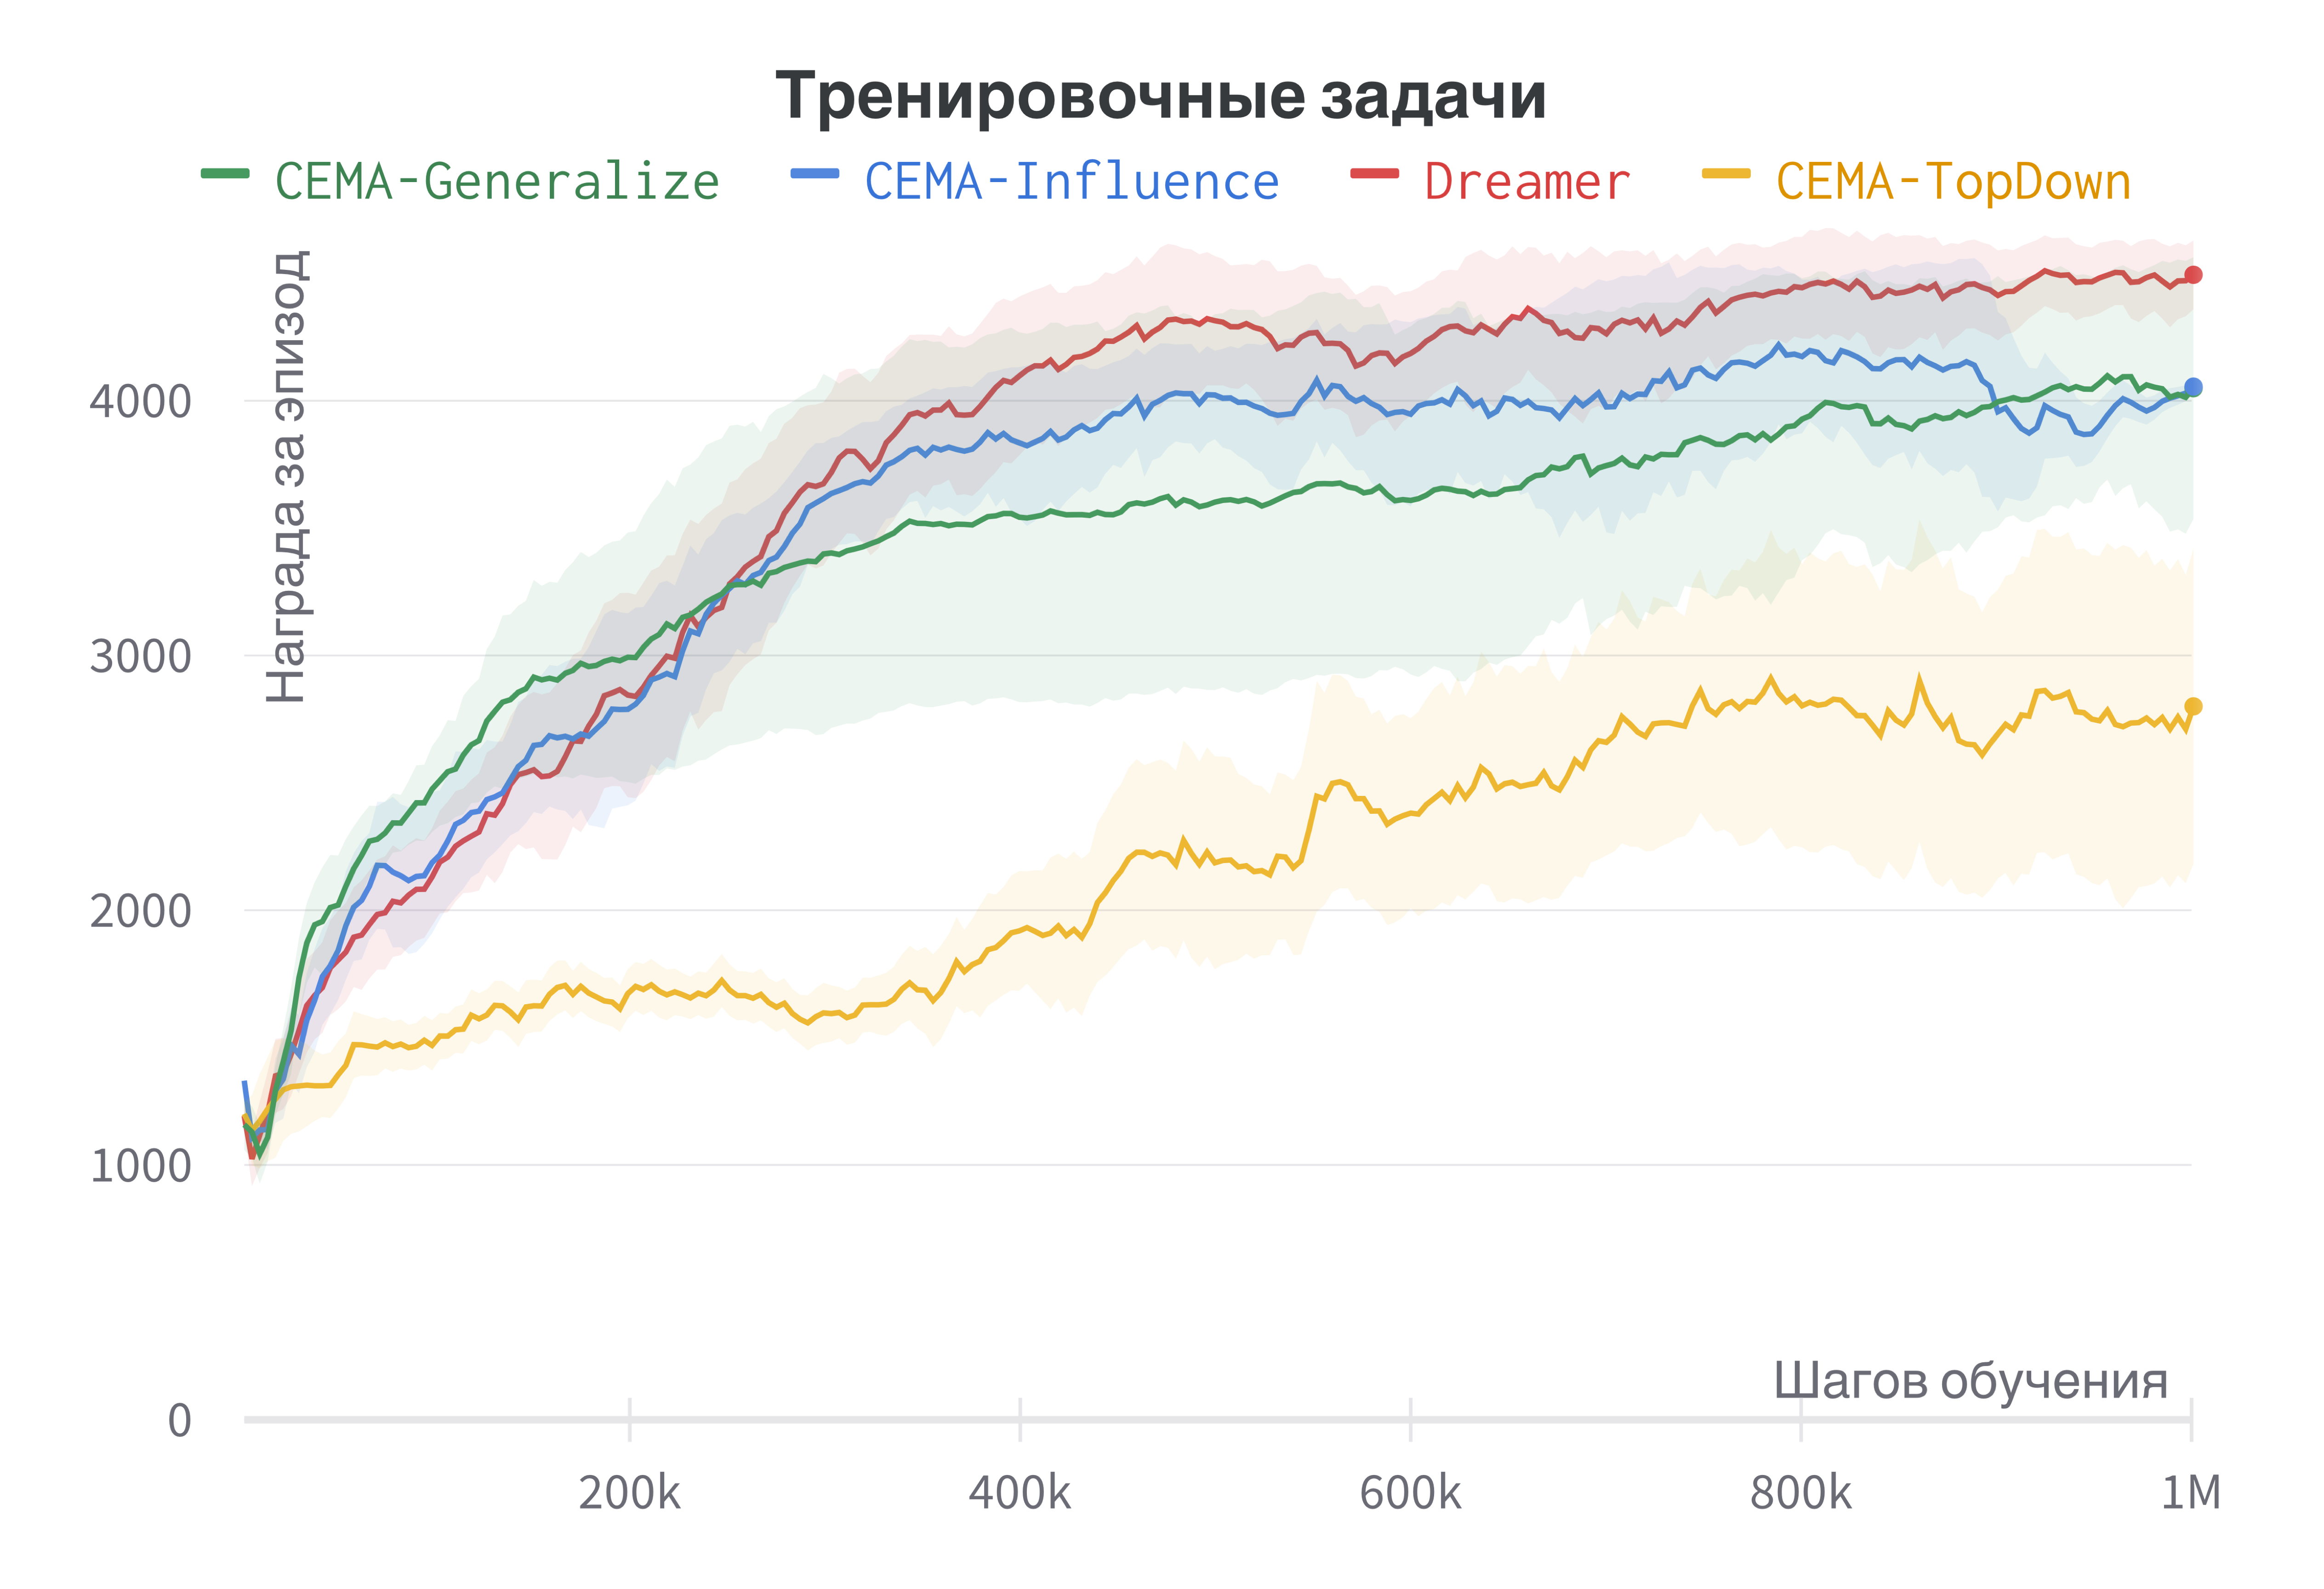
\includegraphics[width=\linewidth]{figures/rdw_train.png}
    \end{subfigure}
    \begin{subfigure}{.47\textwidth}
        \centering
        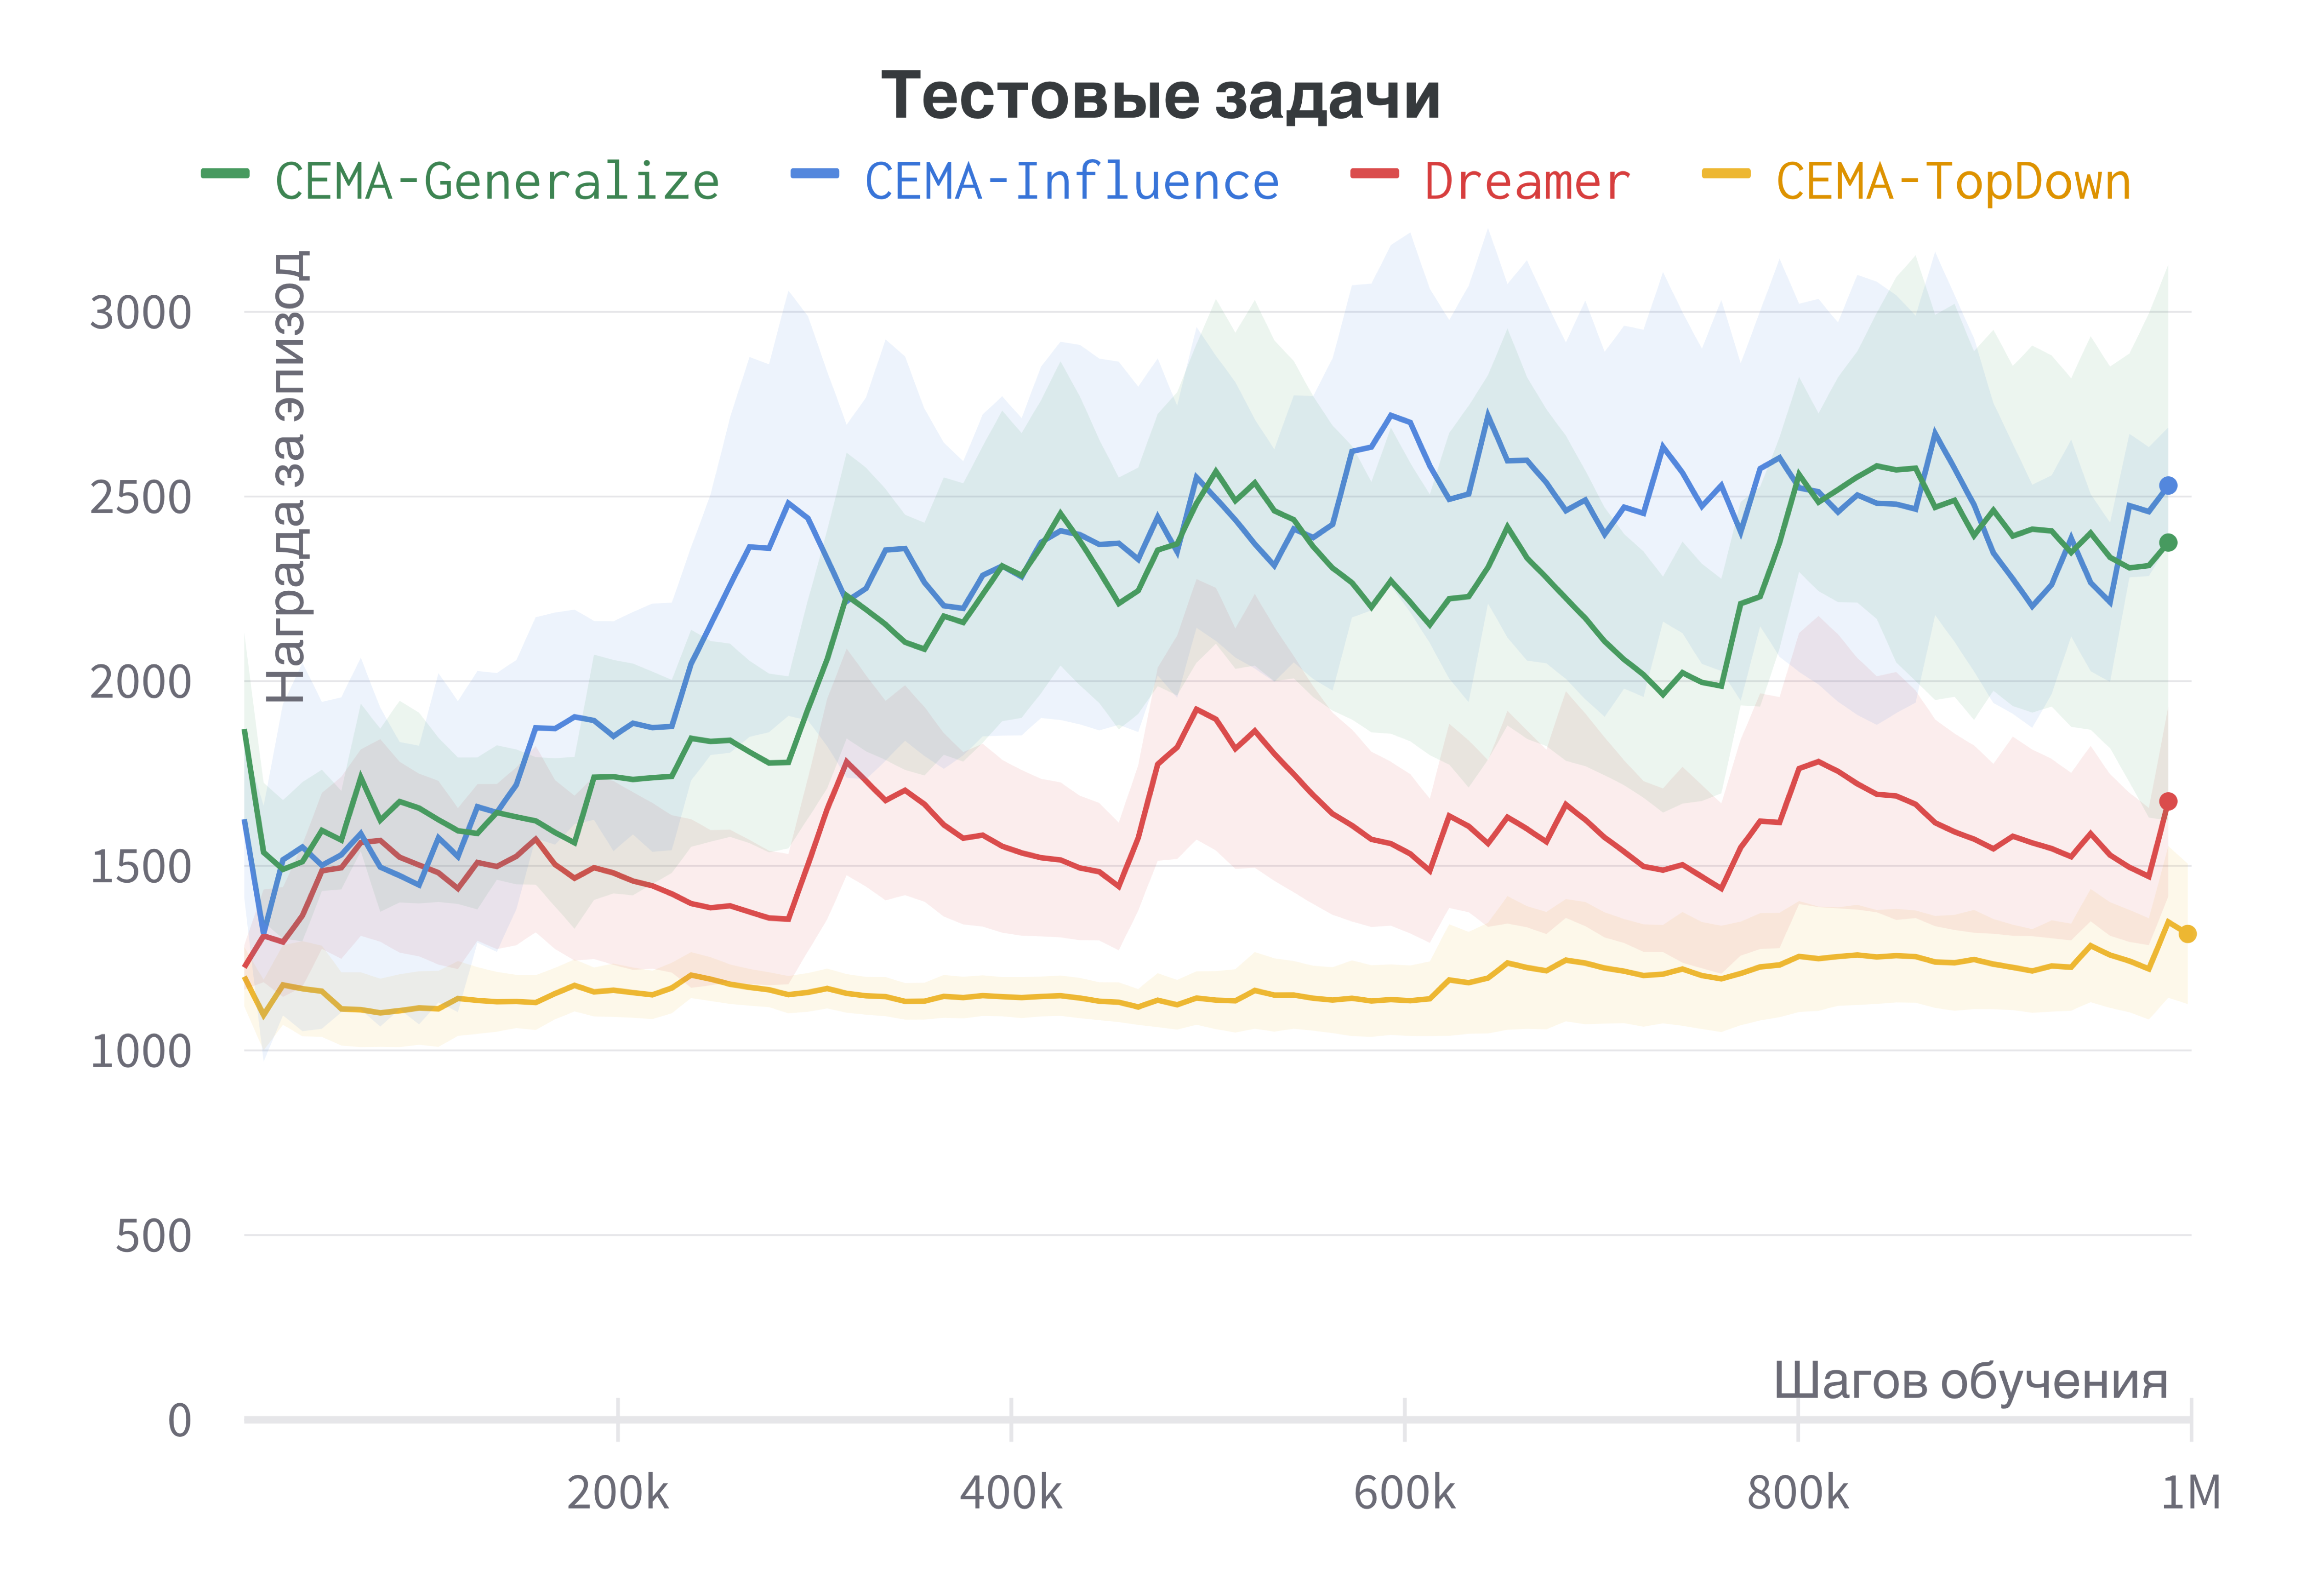
\includegraphics[width=\linewidth]{figures/rdw_test.png}
    \end{subfigure}
    \caption{Графики тренировочного процесса в среде RotatedDrawerOpen.}
    \label{fig:rdw_res}
\end{figure}

На рис. \ref{fig:rdw_res} представлены результаты обучения алгоритмов в среде RotatedDrawerOpen.
Из результатов можно заключить, что опасения, высказанные насчет варианта алгоритма CEMA-TopDown, были справедливы - даже на тренировочных задачах алгоритм показывает себя хуже остальных.
Все предложенные варианты проигрывают базовому алгоритму по скорости обучения на тренировочных задачах.
Однако важно заметить, что для вариантов CEMA-Influence и CEMA-Generalize этот проигрыш не является серьезным - награды в районе $\sim3000$ указывают на то, что алгоритм научился решать задачу, из чего следует что предложенные алгоритмы проигрывают только в скорости решения задач в конкретном эпизоде и при этом алгоритмы выходят по результатам обучения на схожую среднюю награду за эпизод.
Однако на тестовых задачах, два упомянутых алгоритма уверенно превосходят базовый, хоть их результаты и не являются устойчивыми.

\subsection{Эксперименты в наборе сред CasualWorld}
В наборе сред CasualWorld\cite{cw} представлен удобный инструментарий для оценки обобщающих способностей алгоритмов обучения с подкреплением.
Главным преимуществом по сравнению с другими библиотеками для тестирования является удобный интерфейс для параметрического изменения характеристик среды, как визуальных, так и физических.
Аналогично MetaWorld, в CasualWorld содержится набор заранее сконструированных сред и задач в них, а также заранее заданные наборы параметров варьирования задач для тренировки и тестирования алгоритмов.
Сами задачи являются более сложными по сравнению с MetaWorld из-за большей размерности пространства действий, обусловленной конструкцией манипулятора.
Эксперименты в данной среде преследовали цель проверки работы алгоритма в более близких условиях к реальным.

В качестве среды для тестирования была выбрана Pushing.
В наборе задач в этой среде от агента требуется совместить незакреплённый параллелепипед с целью такого же размера, присутствующей на изображении с камер.
Действия являются $9$-мерными векторами $a_t \in \mathbb{R}^9$ и представляют собой координаты трёх пальцев.
Для получения наблюдений используются две камеры, положение и ориентация которых закреплены для всех задач.
Каждая камера предоставляет маску сегментации для манипулятора и объекта, после чего изображения фильтруются, конкатенируются и подаются на вход как $o^r_t$ и $o^o_t$ соответственно.
Каждое получившееся наблюдение является тензором $64 \times 64 \times 6$.
Примеры отдельных изображений среды представлены на рис. \ref{fig:cw}.

\begin{figure}[t]
    \centering
    \begin{subfigure}{.3\textwidth}
        \centering
        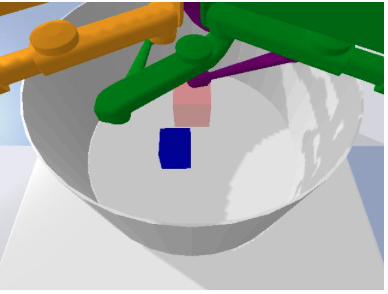
\includegraphics[width=\linewidth]{figures/obs_1.png}
    \end{subfigure}
    \begin{subfigure}{.3\textwidth}
        \centering
        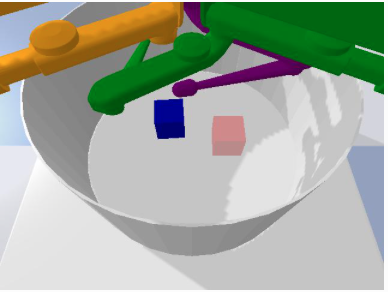
\includegraphics[width=\linewidth]{figures/obs_2.png}
    \end{subfigure}
    \begin{subfigure}{.3\textwidth}
        \centering
        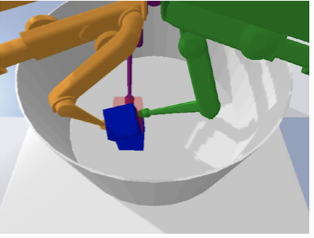
\includegraphics[width=\linewidth]{figures/obs_3.png}
    \end{subfigure}
    \caption{Примеры наблюдений в среде Pushing библиотеки CasualWorld.}
    \label{fig:cw}
\end{figure}

Встроенная функция награды является относительной, то есть зависит от предыдущего состояния среды $\mathcal{R}\left(s_t, s_{t+1}\right)$. 
Поскольку модель функции награды имеет вид $q\left(r_t \mid s_t\right)$, для базового алгоритма задача является достаточно сложной, что выражается в отсутствии прироста показателей качества модели достаточно долгое время при обучении.
Для решения данной проблемы функция награды среды была изменена.
Тогда как механика расчета наград, генерируемых средой, была оставлена нетронутой, агент наблюдает не исходные награды, а сумму всех наград с начала эпизода.
Подобный дизайн награды помогает сделать её менее зависимой от $s_t$, хотя и оставляет зависимость от начального состояния среды $s_0$.
Все представленные результаты для данной среды получены при помощи замены исходных наград $r_t$ на аккумулированные $\hat{r}_t$ в процессе обучения.

В экспериментах используются следующие вариации параметров среды:
\begin{itemize}
    \item Начальное положение объекта $\left(R_{\tau}, \alpha_{\tau}, \frac{h_{\tau}}{2}\right)$
    \item Начальная ориентация объекта $\left(R_{\tau}, \alpha_{\tau}, \frac{h_{\tau}}{2}\right)$
    \item Линейные размеры объекта $\left(l_{\tau}, w_{\tau}, h_{\tau}\right)$
    \item Масса объекта $m_{\tau}$
\end{itemize}
Подробное описание параметров вариации представлено в Таблице \ref{tbl:cw_task_spaces}.

\begin{table}[t]%\small
    \caption{Определение параметров вариации задач в CasualWorld.}
    \label{tbl:cw_task_spaces}
    \centering\medskip%\tabcolsep=2pt%\small
    \begin{tabular}{lrrr}
    \headline
        Параметр вариации
            & \multicolumn{1}{c}{Тренировочные задачи}
            & \multicolumn{1}{c}{Тестовые задачи} \\
    \headline
        {\tt Положение объекта}
            & от $[0.0, - \pi, 0.425]$ & до $[0.11, - \pi, 0.425]$ \\
            & до $[0.11, \pi, 0.425]$ & до $[0.15, \pi, 0.425]$ \\
        {\tt Ориентация объекта}
            & от $[0, 0, -\pi]$ & от $[0, 0, -\pi]$ \\
            & до $[0, 0, \pi]$ & до $[0, 0, \pi]$ \\
        {\tt Размеры объекта}
            & от $[0.075, 0.075, 0.085]$ & от $[0.095, 0.095, 0.085]$ \\
            & до $[0.095, 0.095, 0.085]$ & до $[0.115, 0.115, 0.085]$ \\
        {\tt Масса объекта}
            & от $0.015$ & от $0.045$ \\
            & до $0.045$ & до $0.10$ \\
    \hline
    \end{tabular}
\end{table}

На рис. \ref{fig:cw_res} представлены результаты обучения алгоритмов в среде CasualWorld.
После результатов, полученных на эксперименте в RotatedDrawerWorld, было принято решение исключить более слабый алгоритм CEMA-TopDown из числа рассматриваемых по причине большей сложности CasualWorld.
Как можно заключить из графиков, все испытанные методы уверенно превосходят базовый алгоритм на тренировочных задачах.
На тестовых задачах вариант CEMA-Generalize показывает себя хуже, что может быть проявлением усложнившегося взаимодействия с объектом - вектору влияния слишком сложно предсказать все варианты того, как манипулятор может влиять на объект в любой момент времени.

\begin{figure}[t]
    \centering
    \begin{subfigure}{.47\textwidth}
        \centering
        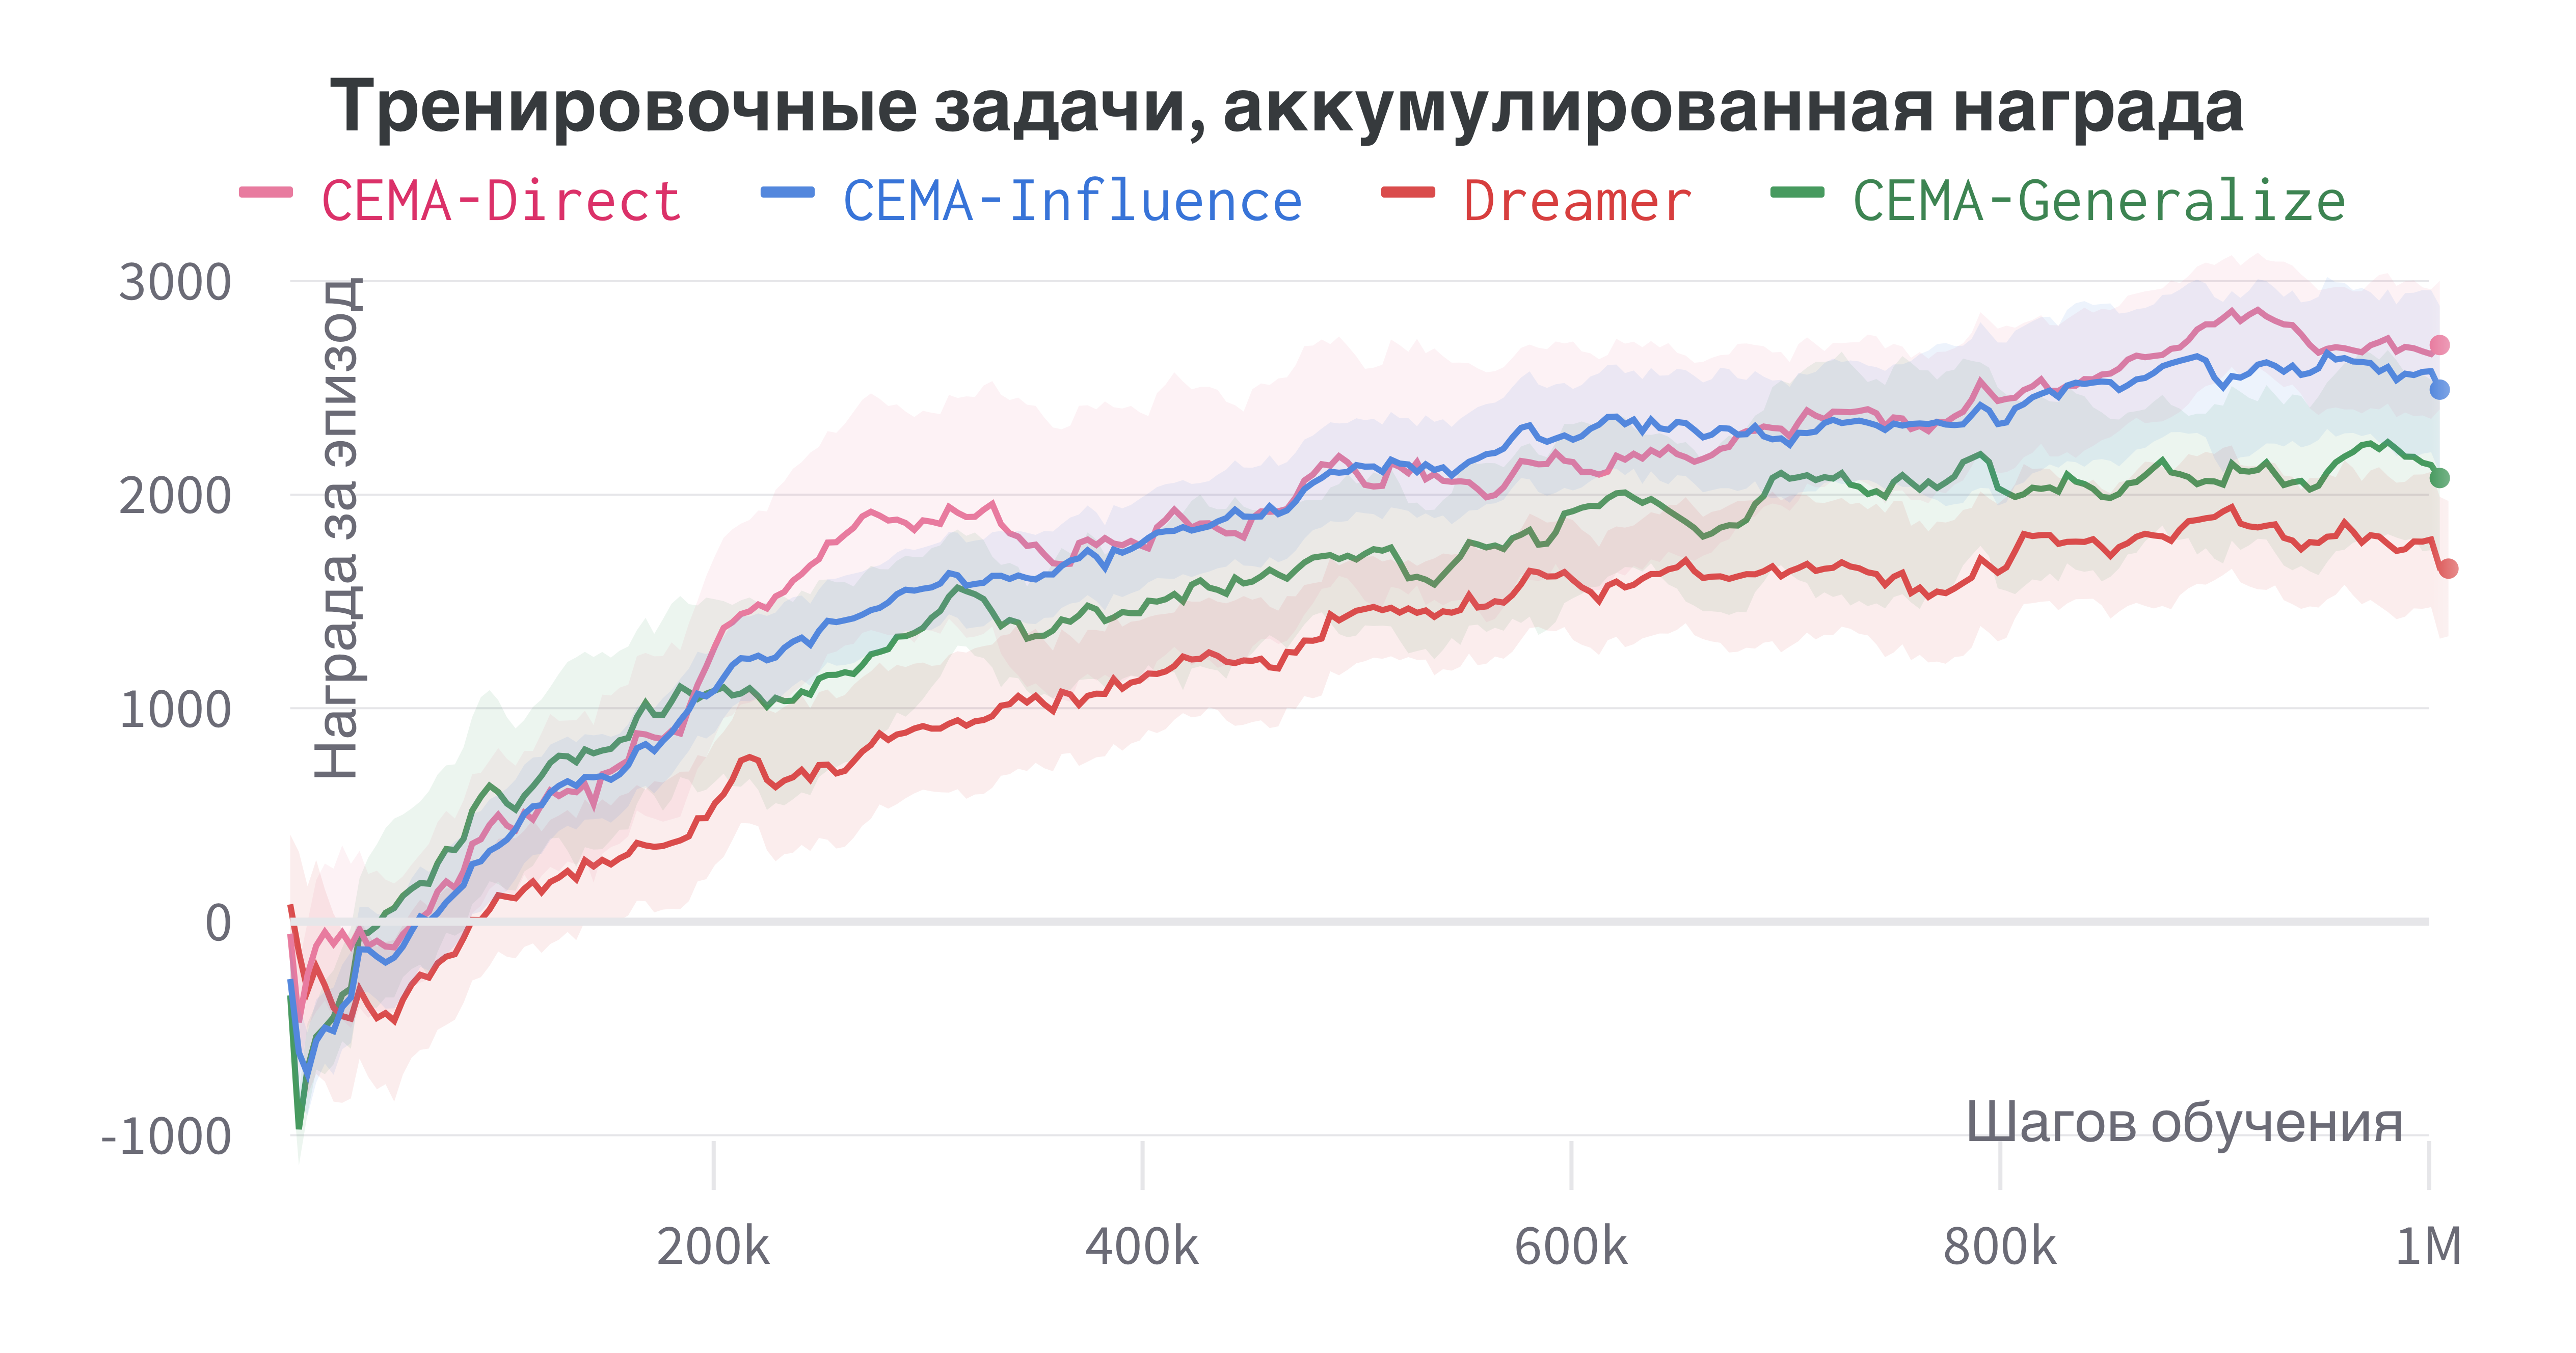
\includegraphics[width=\linewidth]{figures/cw_cum_train.png}
        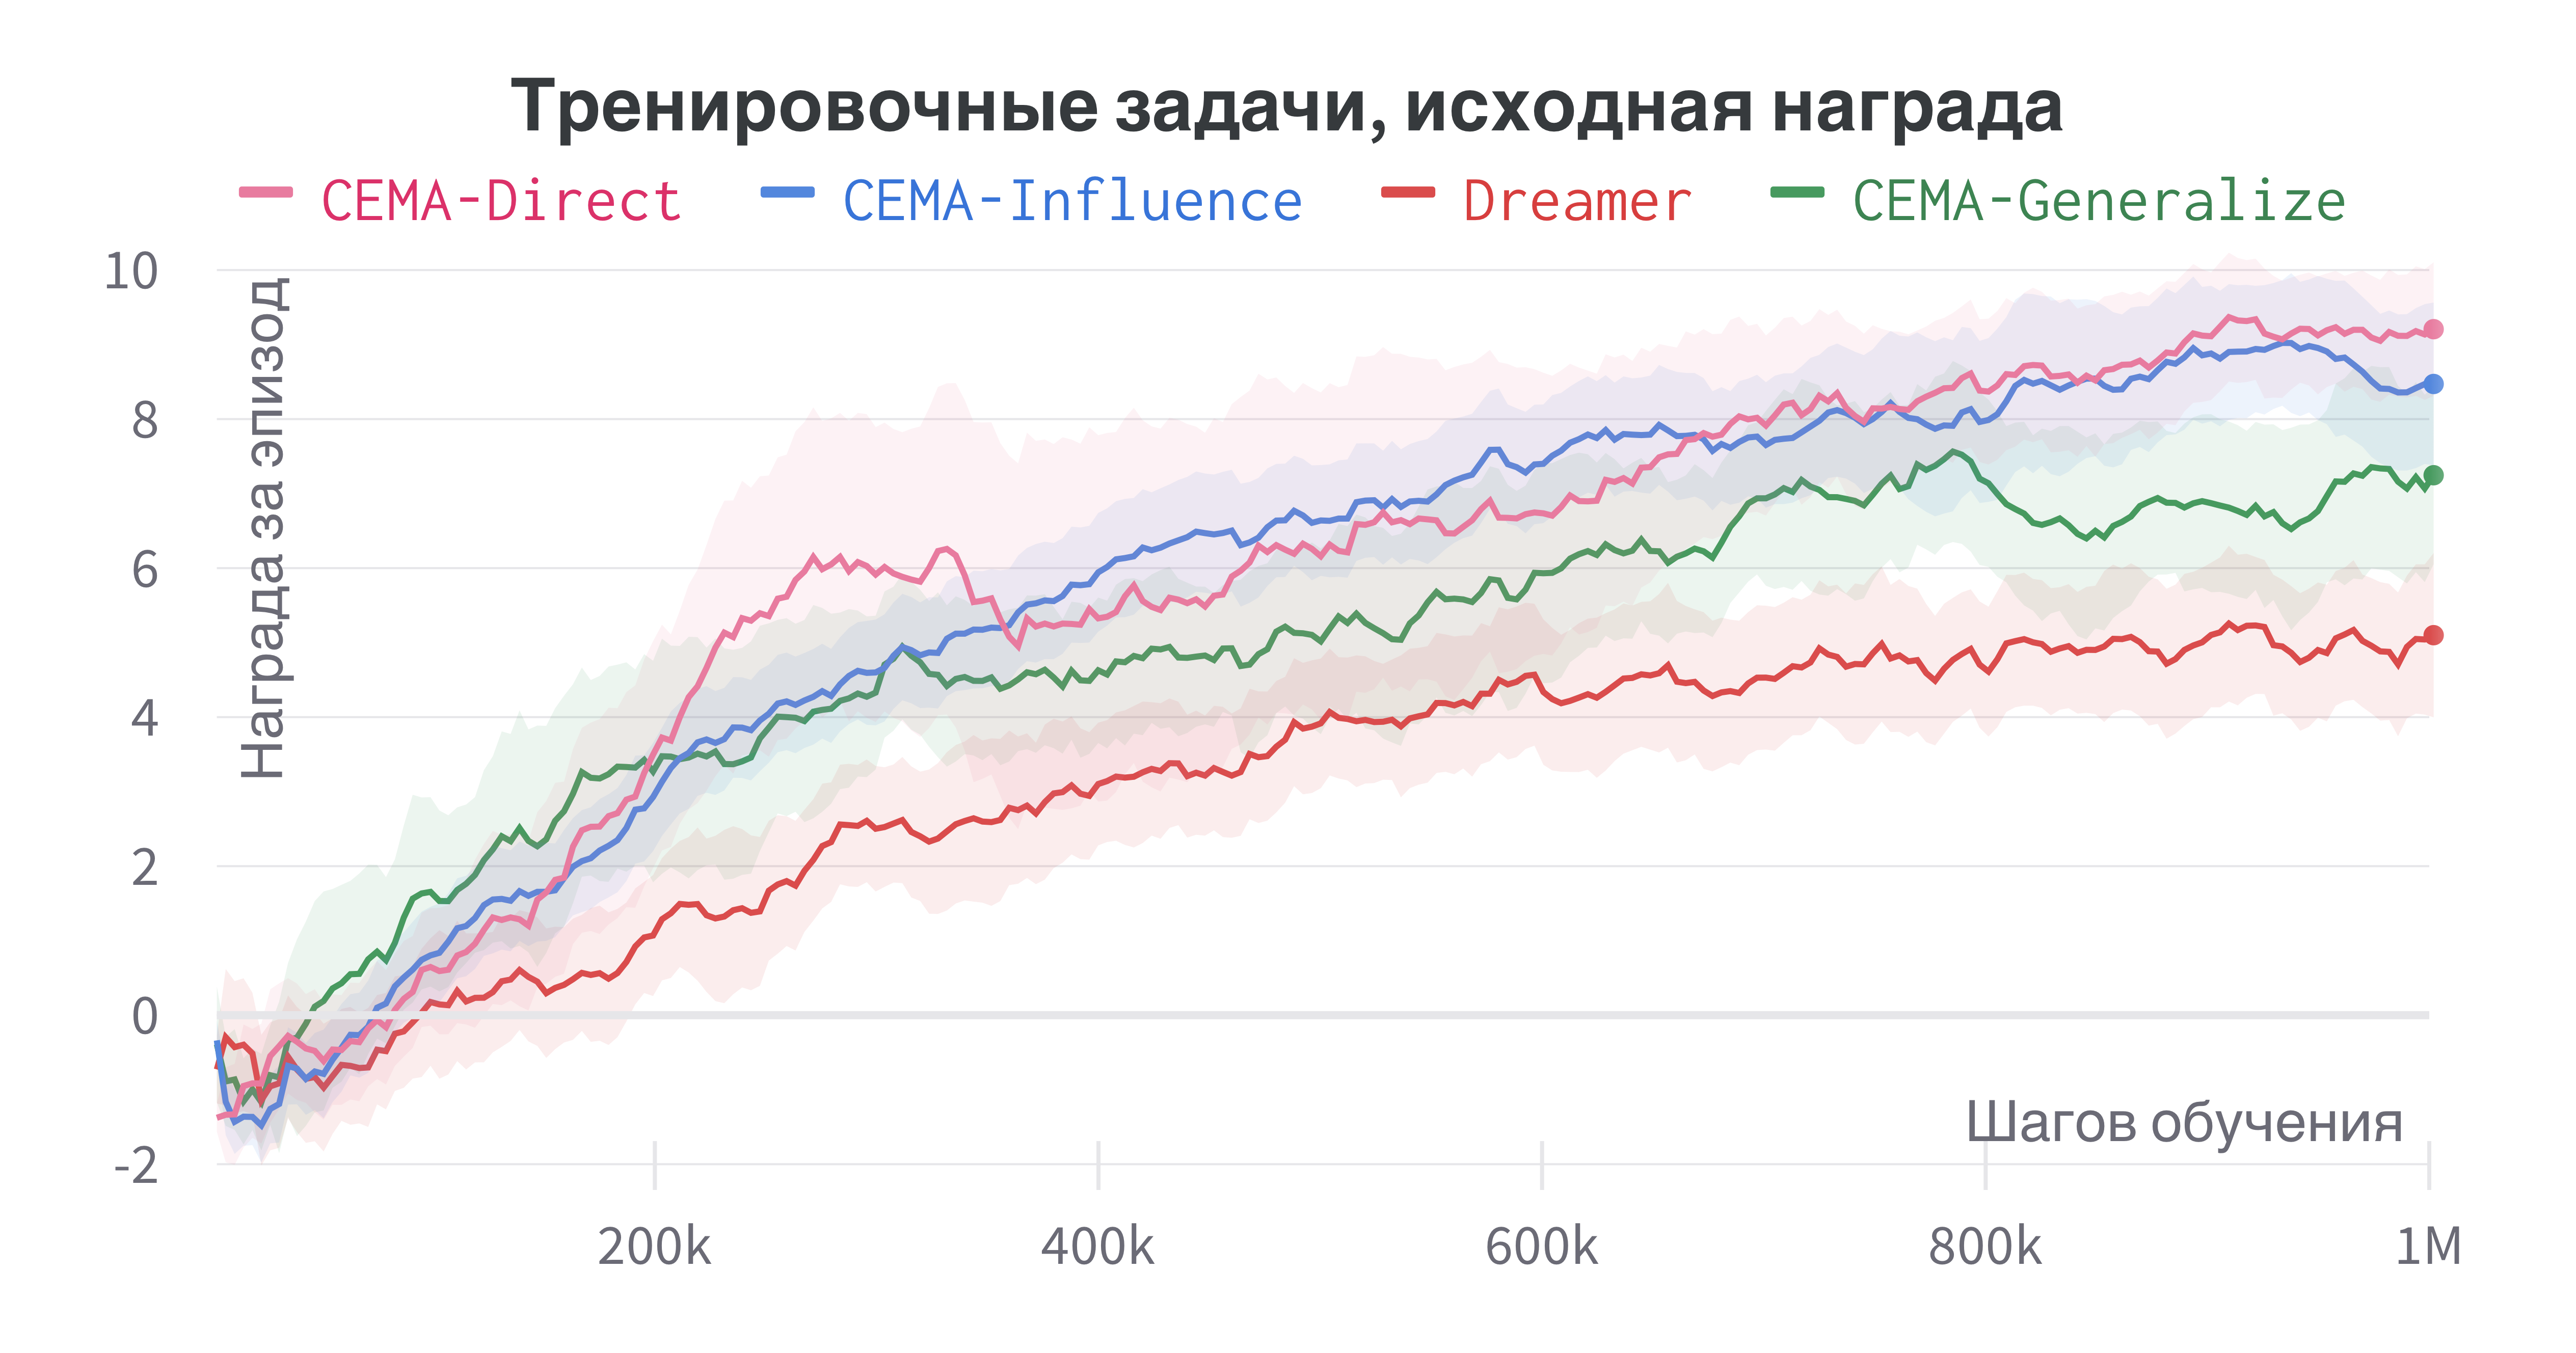
\includegraphics[width=\linewidth]{figures/cw_raw_train.png}
    \end{subfigure}
    \begin{subfigure}{.47\textwidth}
        \centering
        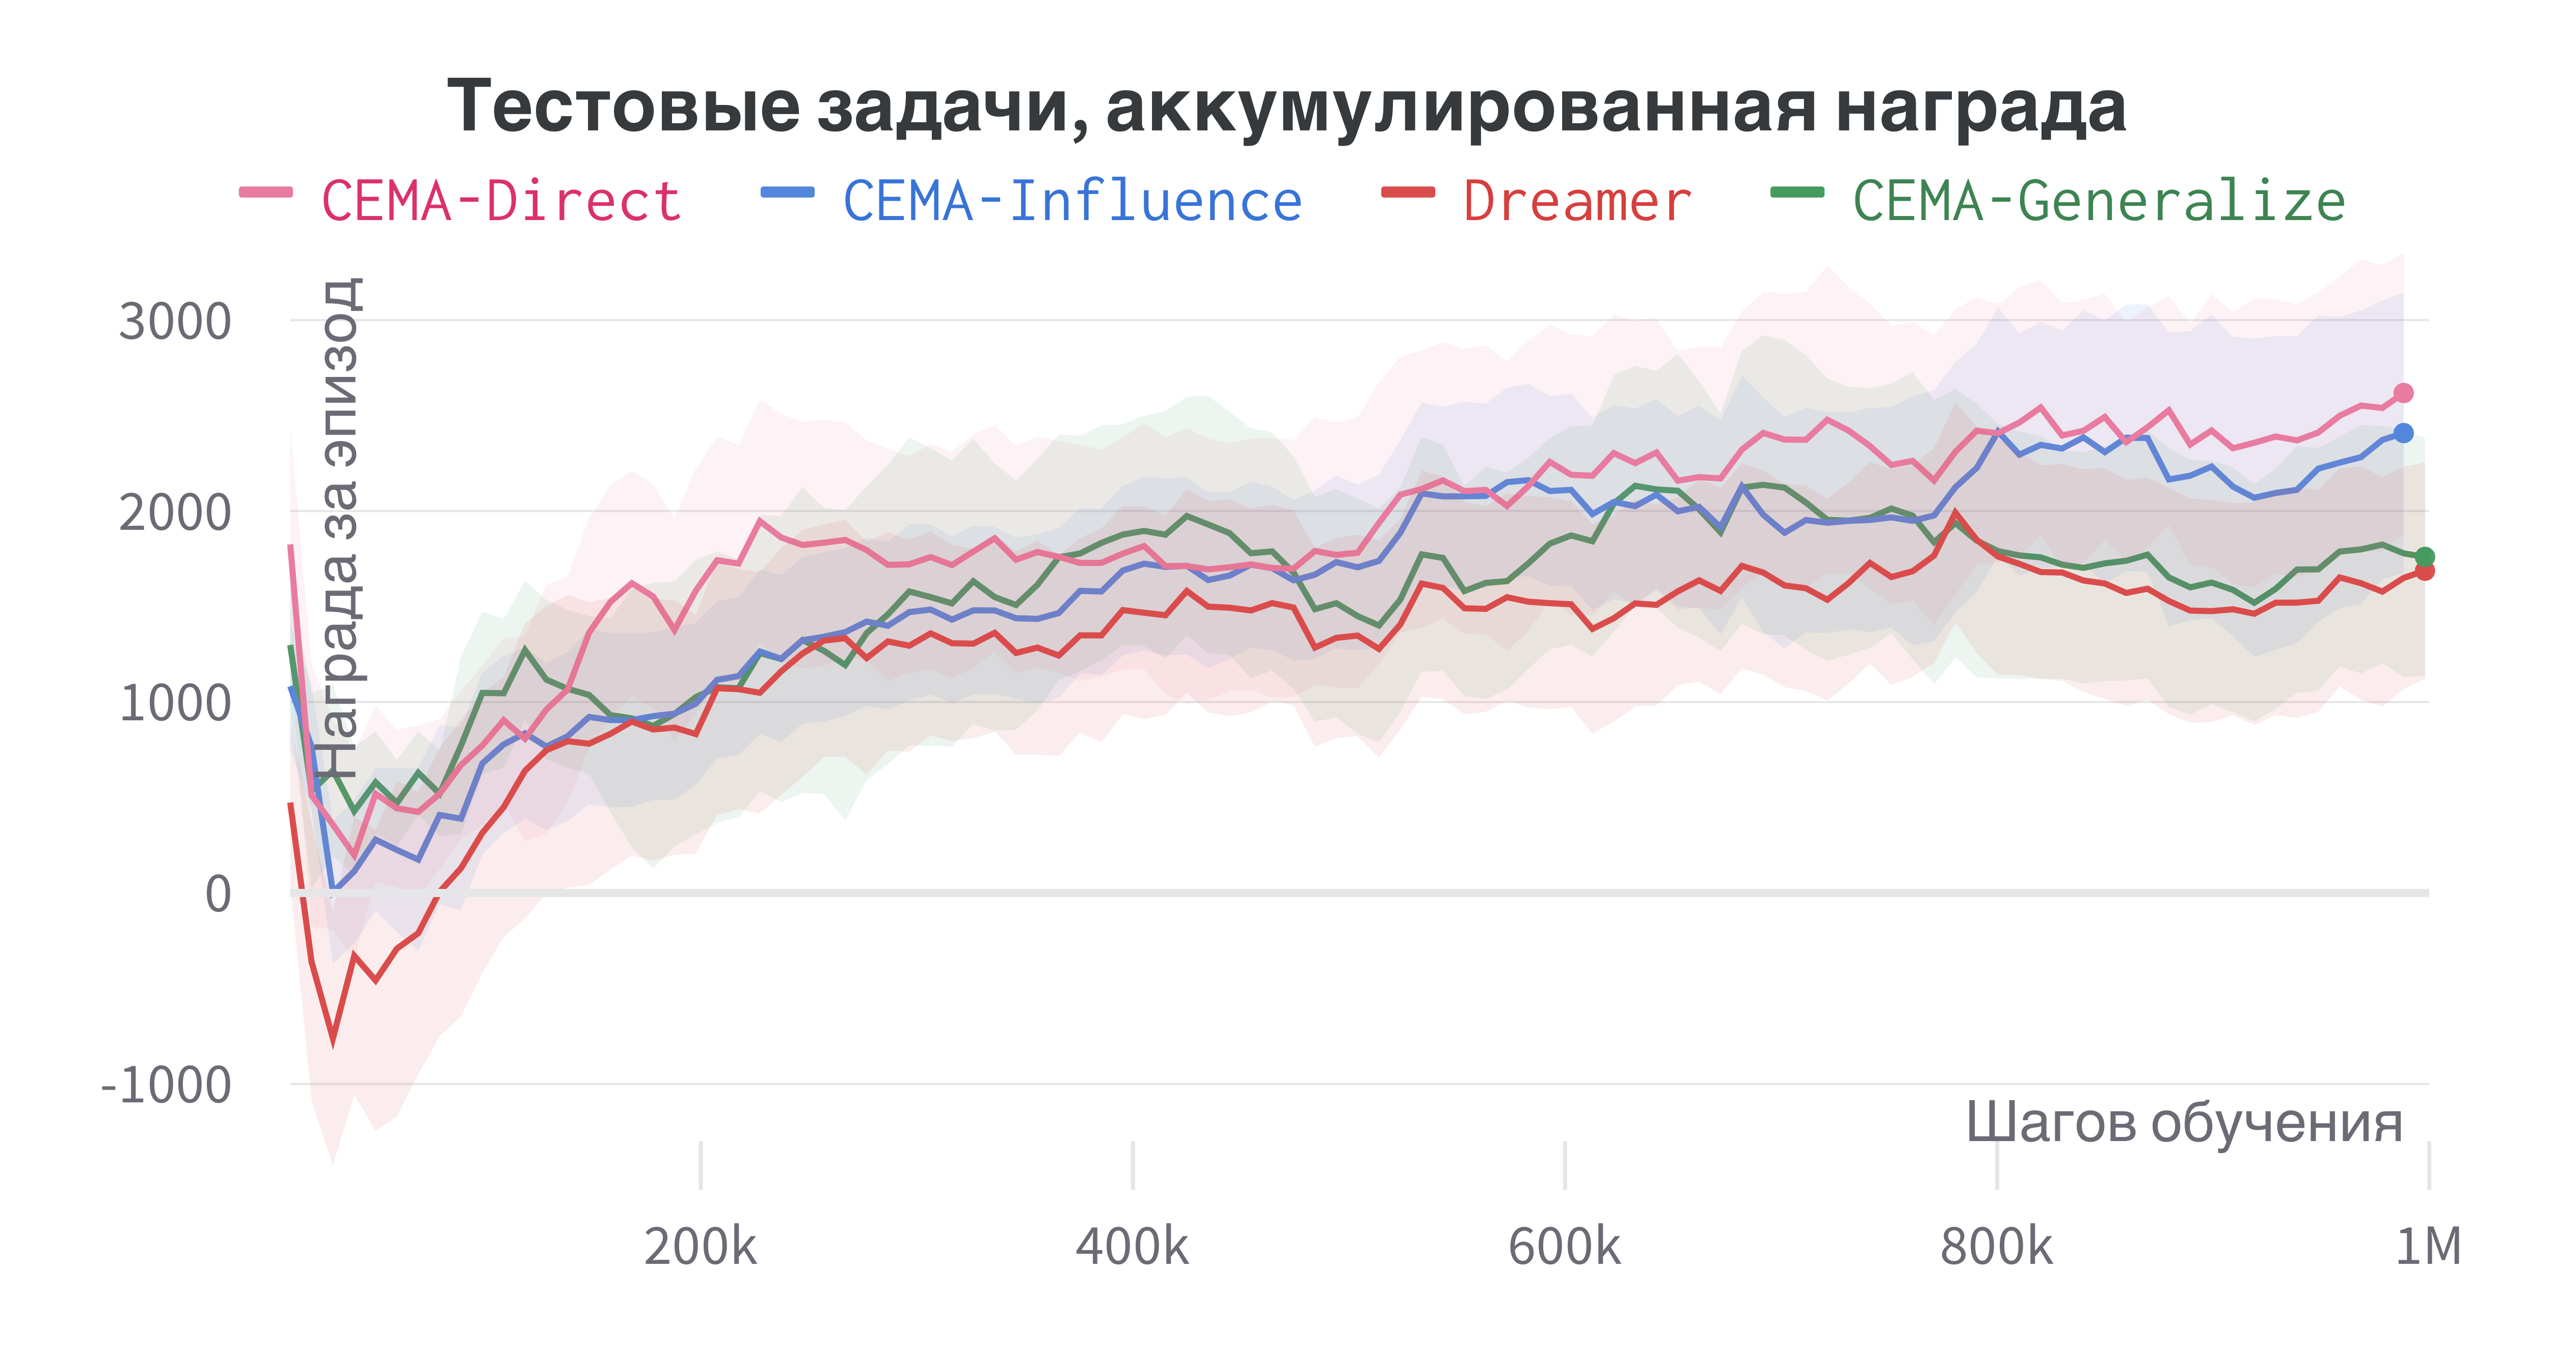
\includegraphics[width=\linewidth]{figures/cw_cum_test.png}
        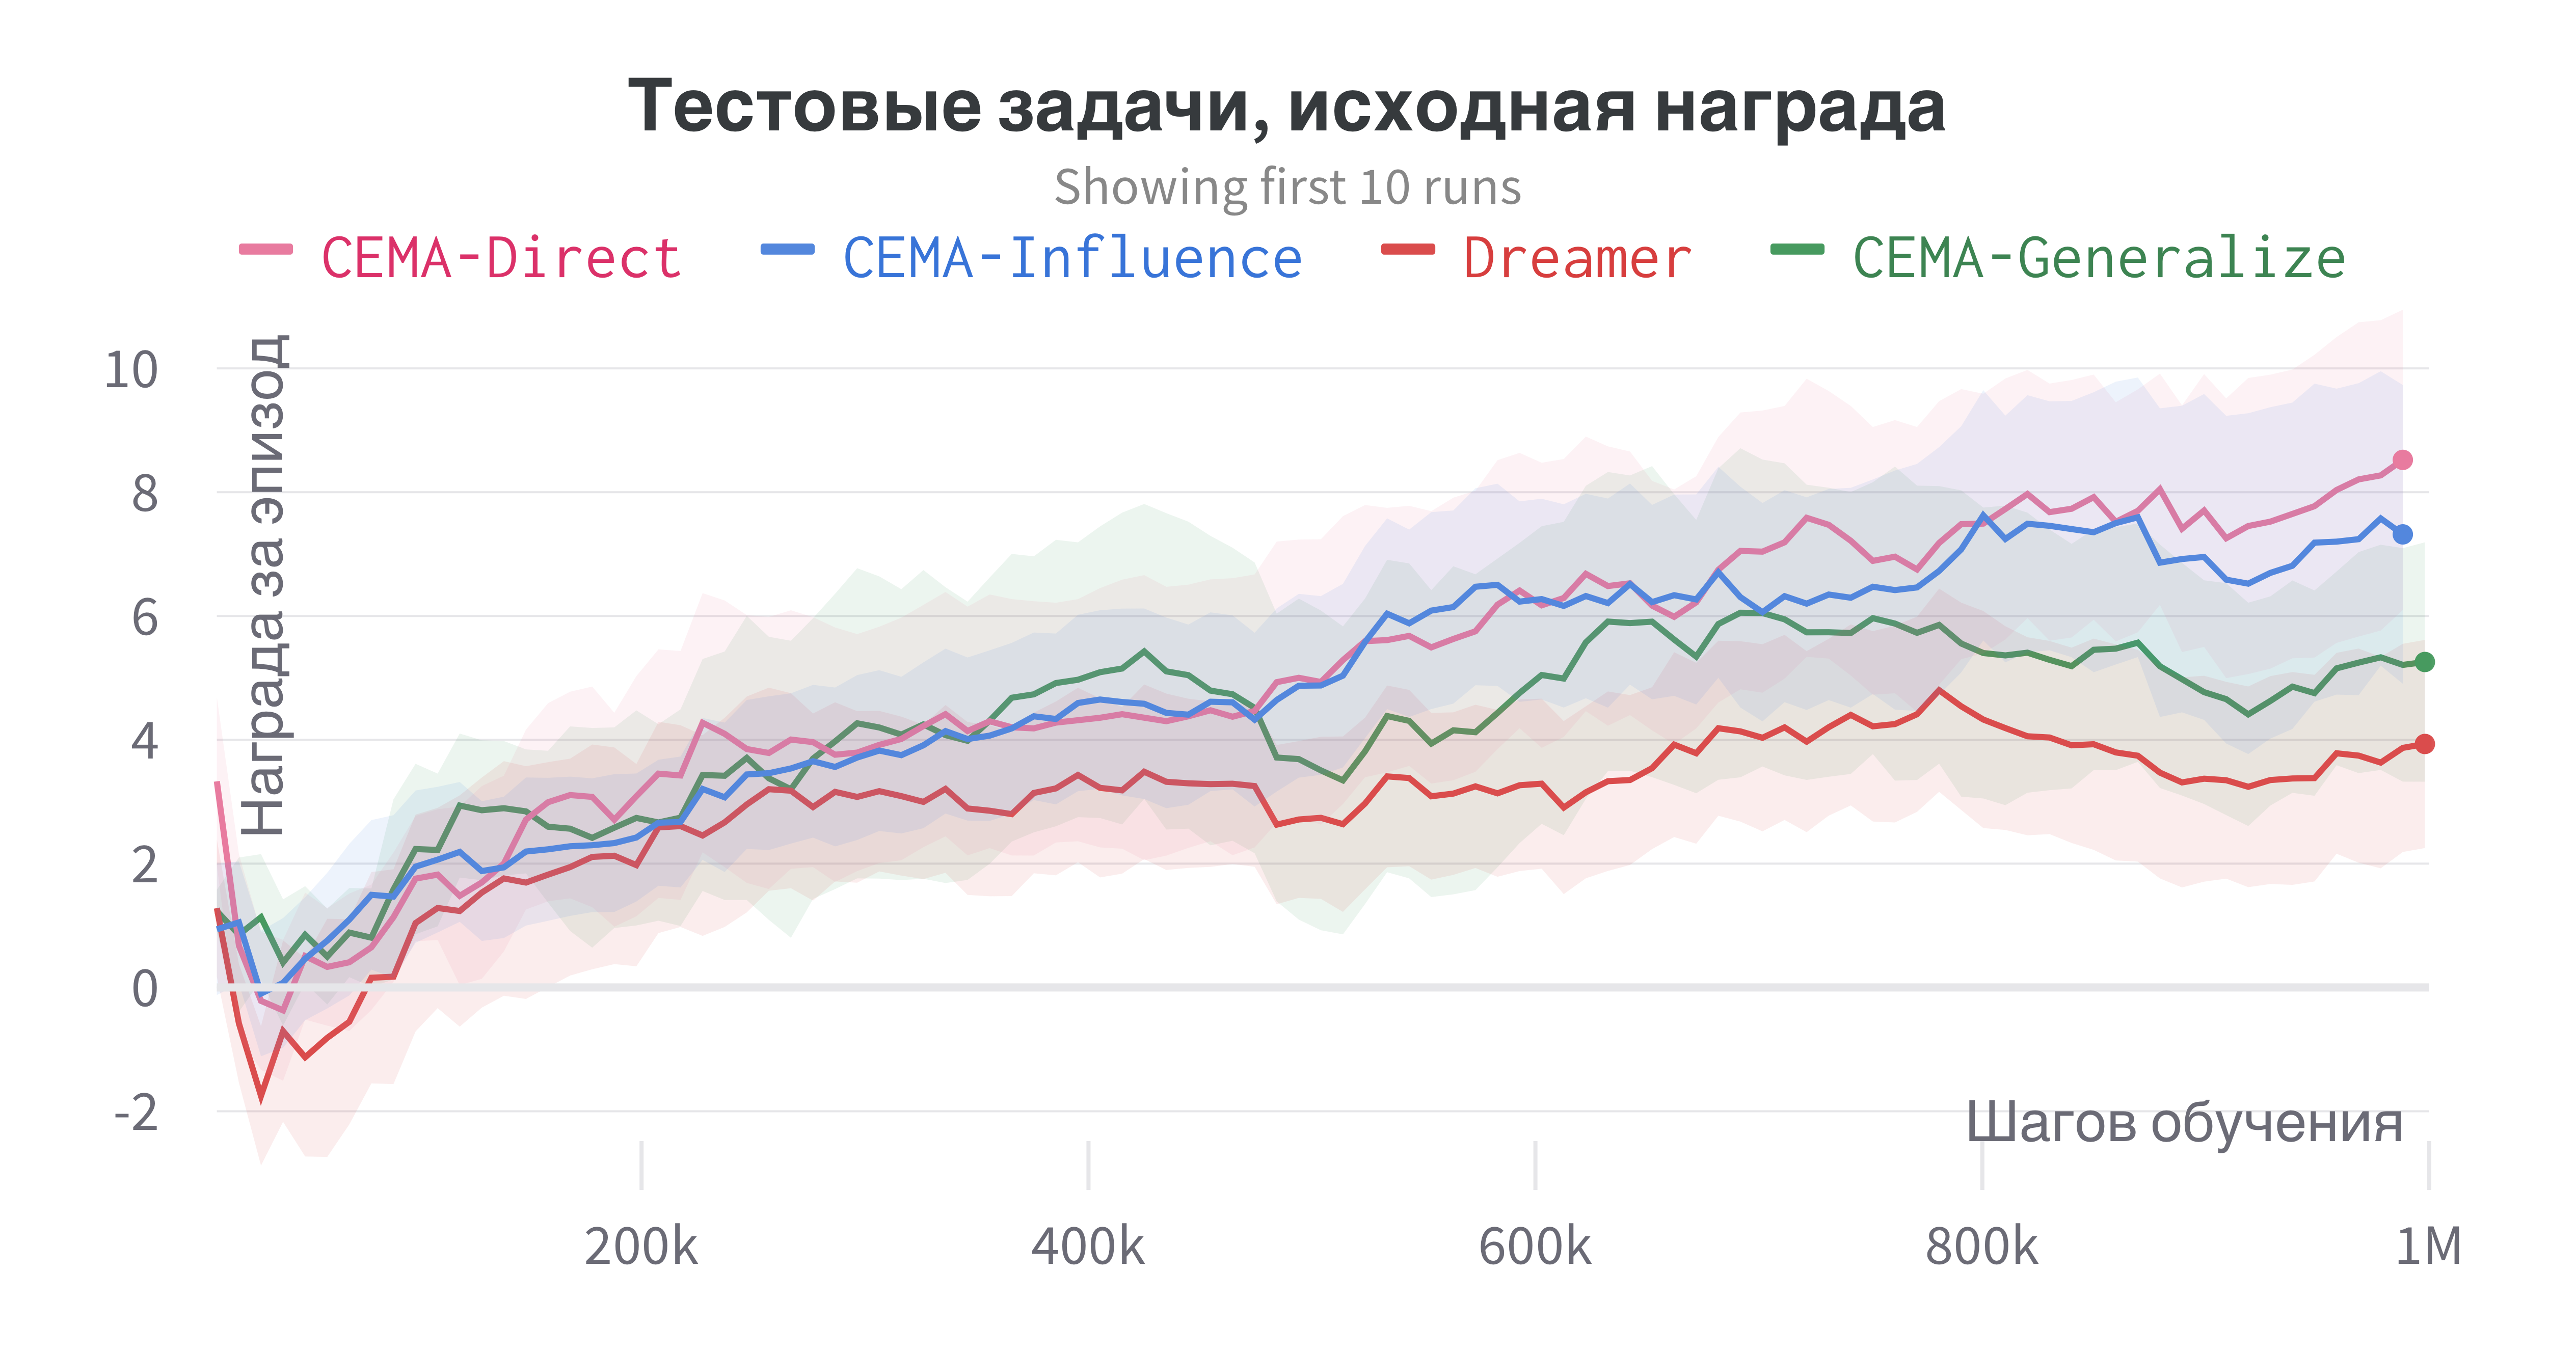
\includegraphics[width=\linewidth]{figures/cw_raw_test.png}
    \end{subfigure}
    \caption{Графики тренировочного процесса в среде Pushing библиотеки CasualWorld.}
    \label{fig:cw_res}
\end{figure}

